\section{Data Flow Diagram}

Data Flow Diagram (DFD) là công cụ mô hình hóa trực quan để biểu diễn luồng dữ liệu trong hệ thống. DFD giúp phân tích cách dữ liệu được xử lý, lưu trữ và truyền tải giữa các thực thể, tiến trình và kho dữ liệu.

\subsection{DFD ngữ cảnh}

DFD ngữ cảnh (Context Diagram) cung cấp cái nhìn tổng quan về hệ thống BarberGo và các thực thể bên ngoài tương tác với nó. Sơ đồ này thể hiện hệ thống như một tiến trình duy nhất và mô tả các luồng dữ liệu chính giữa hệ thống và các actor bên ngoài.

\begin{figure}[H]
    \centering
    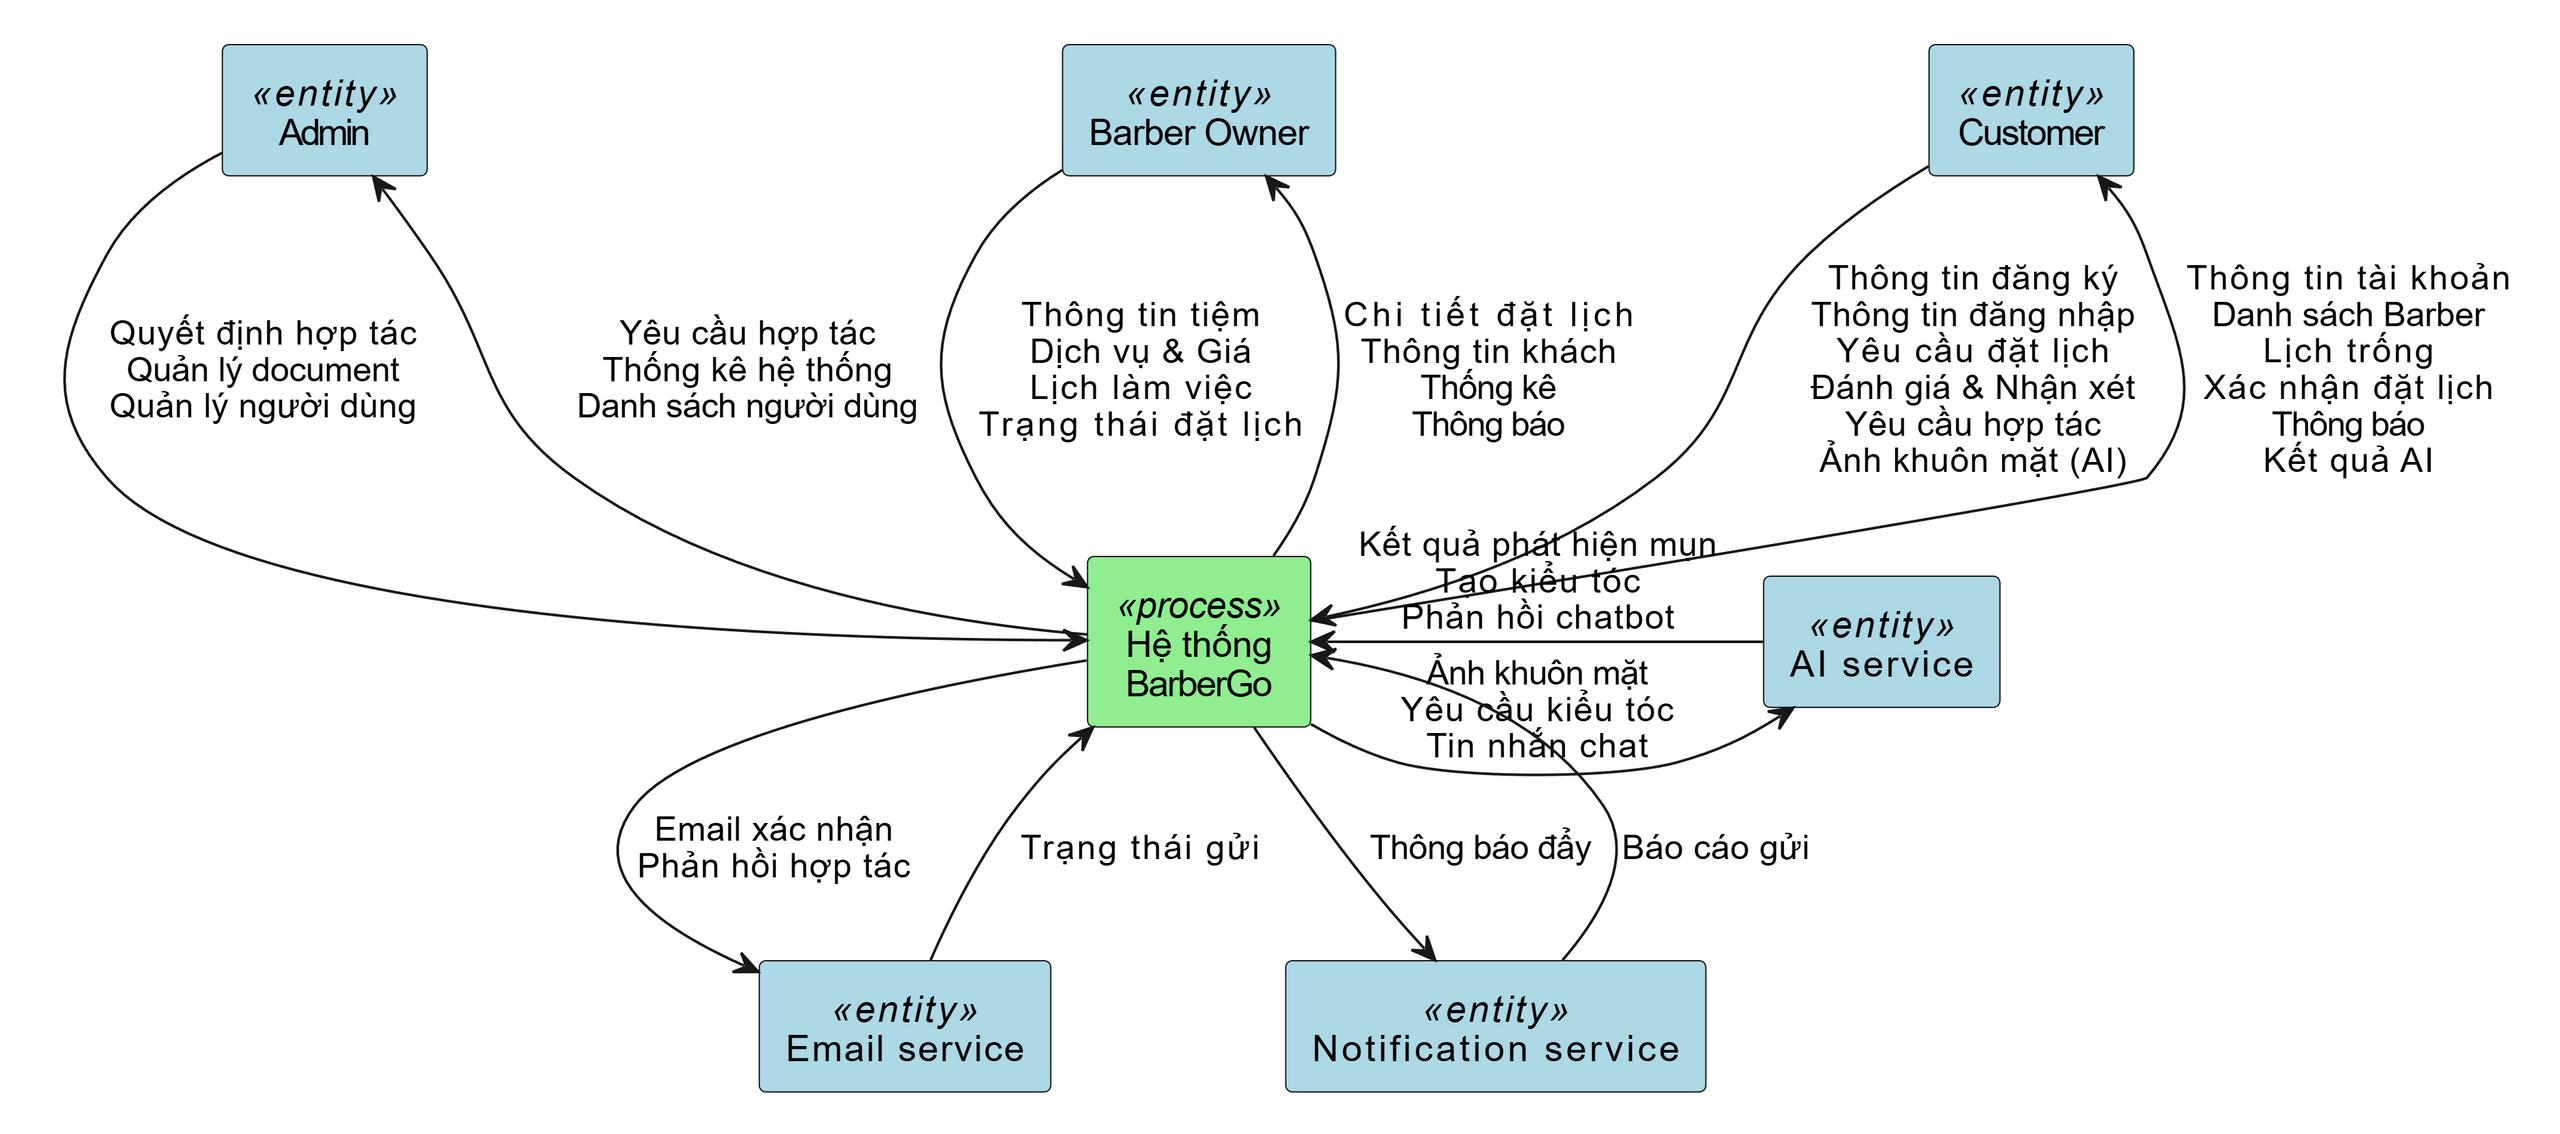
\includegraphics[width=1.0\textwidth]{figures/dfdc.jpg}
    \caption{DFD ngữ cảnh}
    \label{fig:dfdc}
\end{figure}

Các thực thể bên ngoài tương tác với hệ thống bao gồm:
\begin{itemize}
    \item \textbf{Customer:} Đăng ký tài khoản, tìm kiếm barber, đặt lịch, sử dụng tính năng AI, đánh giá dịch vụ và gửi yêu cầu hợp tác
    \item \textbf{Barber Owner:} Quản lý thông tin tiệm, dịch vụ, lịch làm việc và xử lý đặt lịch từ khách hàng
    \item \textbf{Admin:} Quản lý người dùng, duyệt yêu cầu hợp tác, cập nhật knowledge base và xem thống kê hệ thống
    \item \textbf{AI Service:} Xử lý phát hiện mụn, tạo kiểu tóc và cung cấp chatbot RAG
    \item \textbf{Email Service:} Gửi email xác nhận và phản hồi yêu cầu hợp tác
    \item \textbf{Notification Service (FCM):} Gửi thông báo đẩy đến thiết bị di động
\end{itemize}

\subsection{DFD cấp 0}

DFD cấp 0 phân rã hệ thống BarberGo thành các tiến trình chức năng chính và các kho dữ liệu tương ứng. Mỗi tiến trình đại diện cho một module nghiệp vụ độc lập.

\begin{figure}[H]
    \centering
    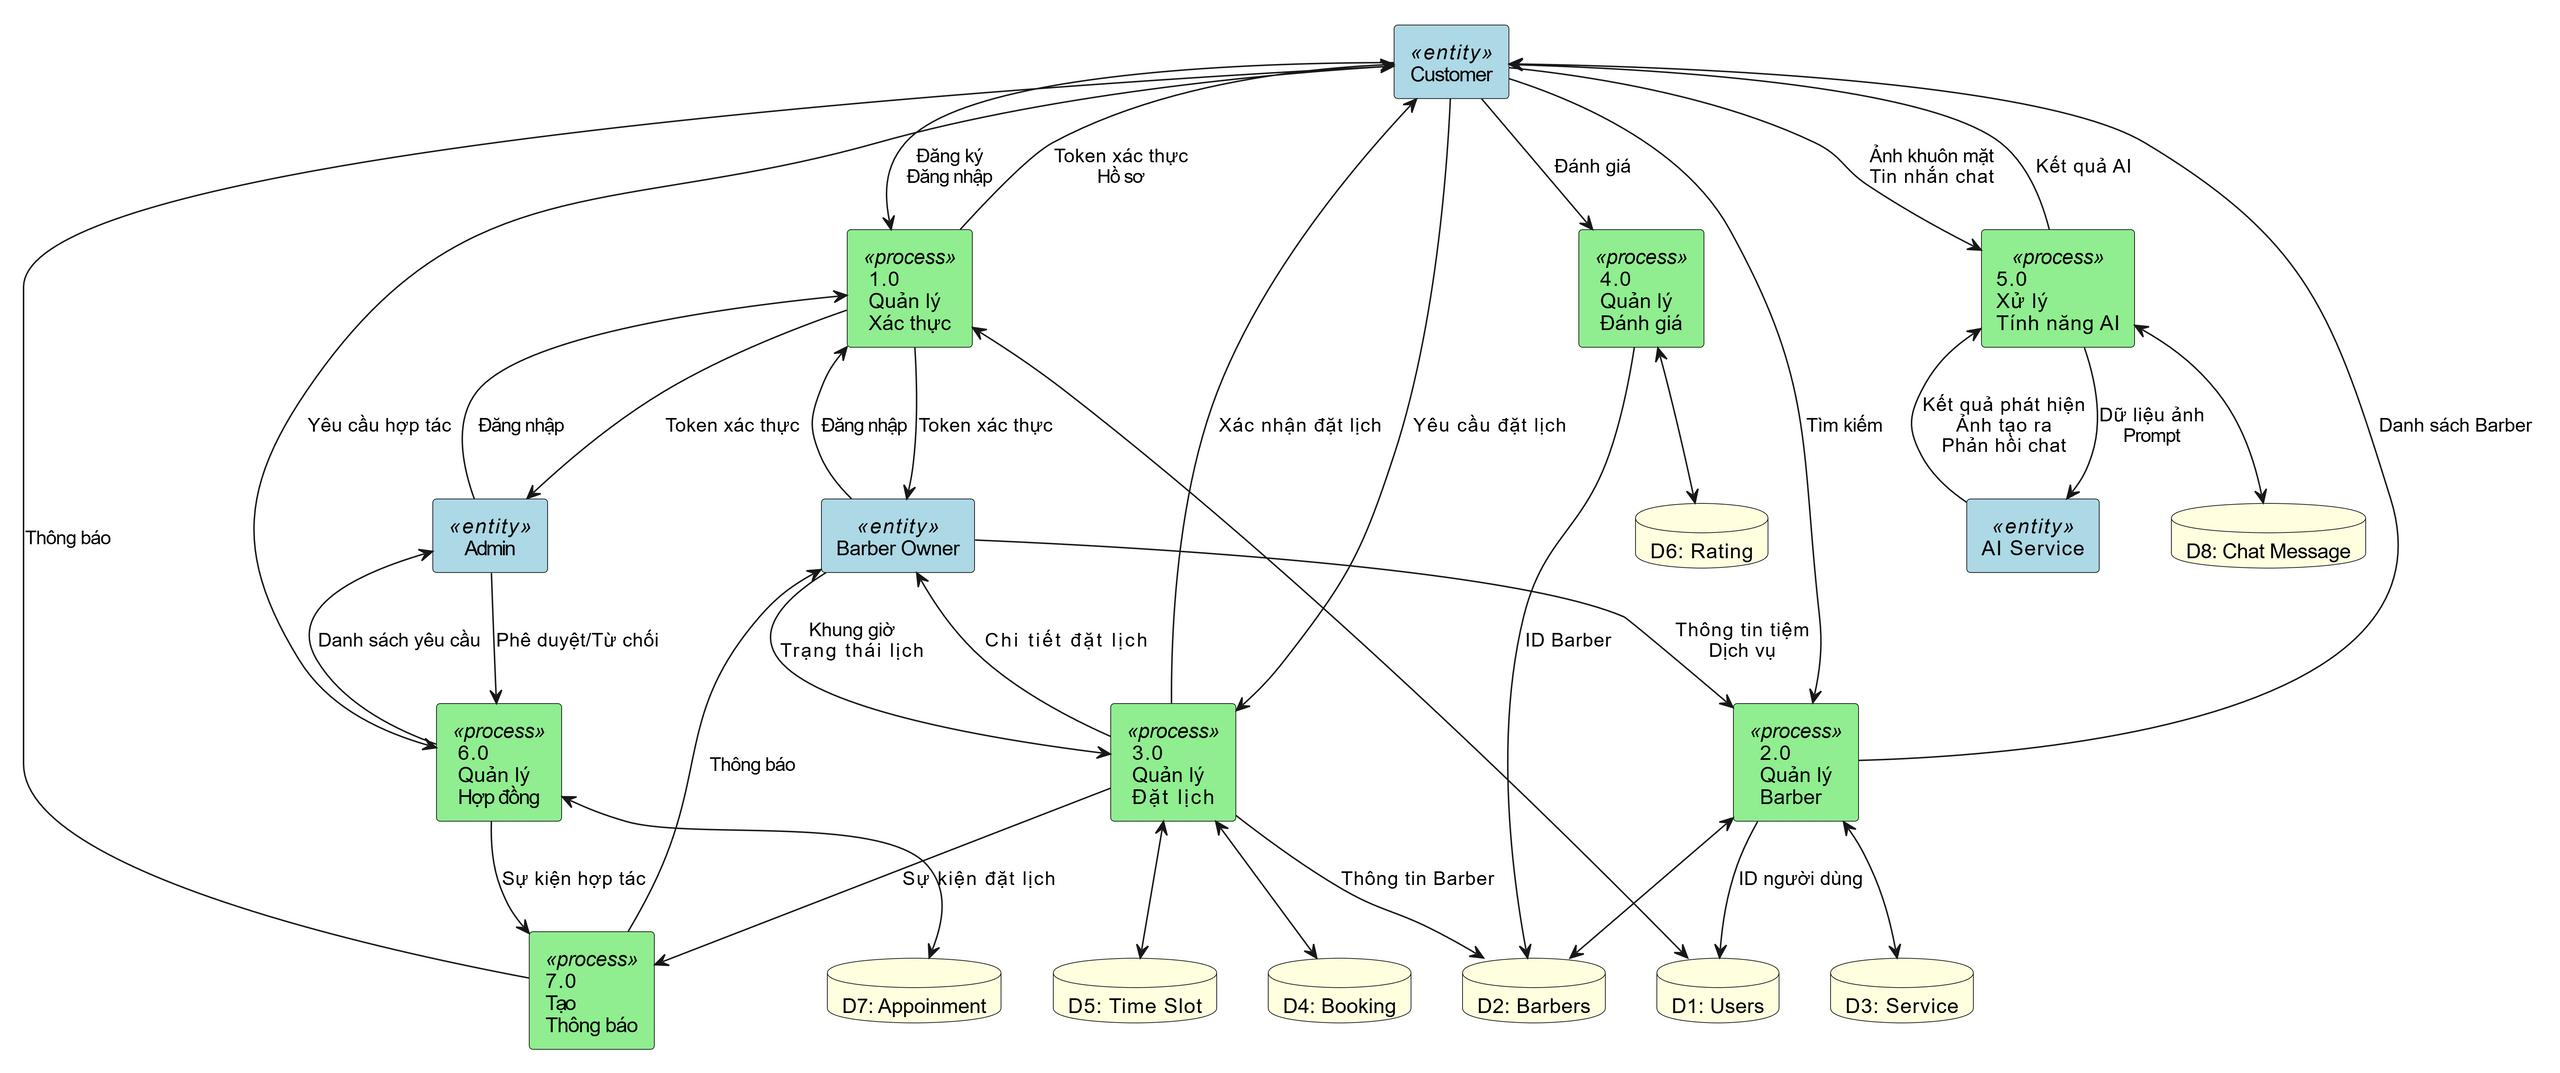
\includegraphics[width=0.85\textwidth]{figures/dfd0.jpg}
    \caption{DFD cấp 0}
    \label{fig:dfd0}
\end{figure}

Các tiến trình chính trong hệ thống:
\begin{itemize}
    \item \textbf{1.0 Quản lý Xác thực:} Xử lý đăng ký, đăng nhập, quản lý hồ sơ và đăng xuất
    \item \textbf{2.0 Quản lý Barber:} Quản lý thông tin tiệm cắt tóc, dịch vụ và giờ làm việc
    \item \textbf{3.0 Quản lý Đặt lịch:} Xử lý đặt lịch, quản lý khung giờ và xác nhận/hủy lịch hẹn
    \item \textbf{4.0 Quản lý Đánh giá:} Thu thập và hiển thị đánh giá từ khách hàng
    \item \textbf{5.0 Xử lý Tính năng AI:} Tích hợp phát hiện mụn, tạo kiểu tóc và chatbot RAG
    \item \textbf{6.0 Quản lý Hợp tác:} Xử lý yêu cầu hợp tác từ khách hàng và phản hồi từ admin
    \item \textbf{7.0 Tạo Thông báo:} Gửi thông báo đẩy và email cho người dùng
\end{itemize}

Các kho dữ liệu chính:
\begin{itemize}
    \item \textbf{D1: Users} - Lưu trữ thông tin người dùng (khách hàng, barber owner, admin)
    \item \textbf{D2: Barbers} - Thông tin tiệm cắt tóc
    \item \textbf{D3: Services} - Dịch vụ và giá cả
    \item \textbf{D4: Bookings} - Lịch hẹn đã đặt
    \item \textbf{D5: Time Slots} - Khung giờ làm việc
    \item \textbf{D6: Ratings} - Đánh giá từ khách hàng
    \item \textbf{D7: Appointments} - Yêu cầu hợp tác
    \item \textbf{D8: Chat Messages} - Lịch sử chat với bot
    \item \textbf{D9: Documents} - Knowledge base cho RAG
\end{itemize}

\subsection{DFD Cấp 1 - Xác thực}

DFD cấp 1 cho module Xác thực mô tả chi tiết các tiến trình con liên quan đến quản lý tài khoản người dùng.

\begin{figure}[H]
    \centering
    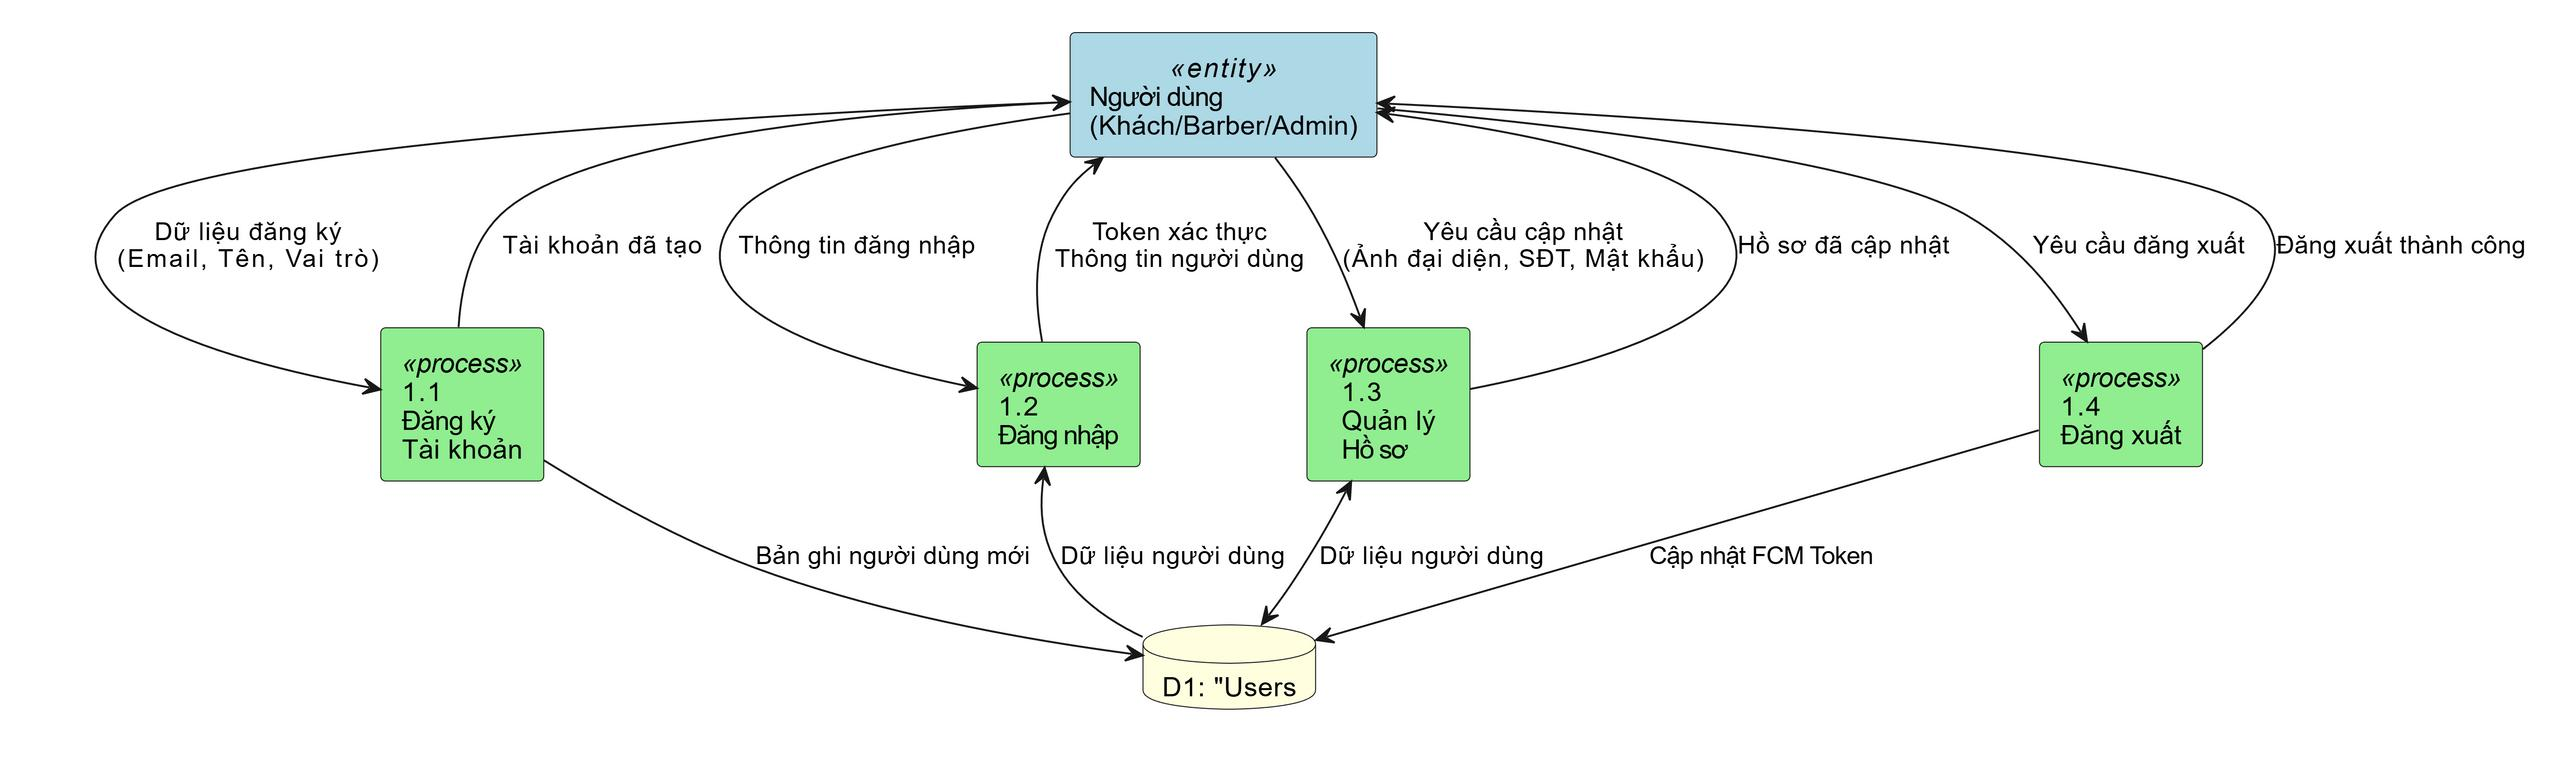
\includegraphics[width=0.7\textwidth]{figures/dfd1_auth.jpg}
    \caption{DFD cấp 1 - Xác thực}
    \label{fig:dfd1_auth}
\end{figure}

Các tiến trình con:
\begin{itemize}
    \item \textbf{1.1 Đăng ký Tài khoản:} Tạo tài khoản mới với email, tên và vai trò (customer/barber/admin). Dữ liệu được validate và lưu vào D1: Users
    \item \textbf{1.2 Đăng nhập:} Xác thực thông tin đăng nhập, truy vấn D1: Users và trả về JWT token cùng thông tin người dùng
    \item \textbf{1.3 Quản lý Hồ sơ:} Cho phép người dùng cập nhật thông tin cá nhân như ảnh đại diện, số điện thoại và mật khẩu
    \item \textbf{1.4 Đăng xuất:} Xử lý đăng xuất và cập nhật FCM token trong D1: Users để ngừng nhận thông báo
\end{itemize}

\subsection{DFD Cấp 1 - Quản lý cửa tiệm}

DFD cấp 1 cho module Quản lý Barber chi tiết hóa các tiến trình liên quan đến quản lý thông tin tiệm cắt tóc và dịch vụ.

\begin{figure}[H]
    \centering
    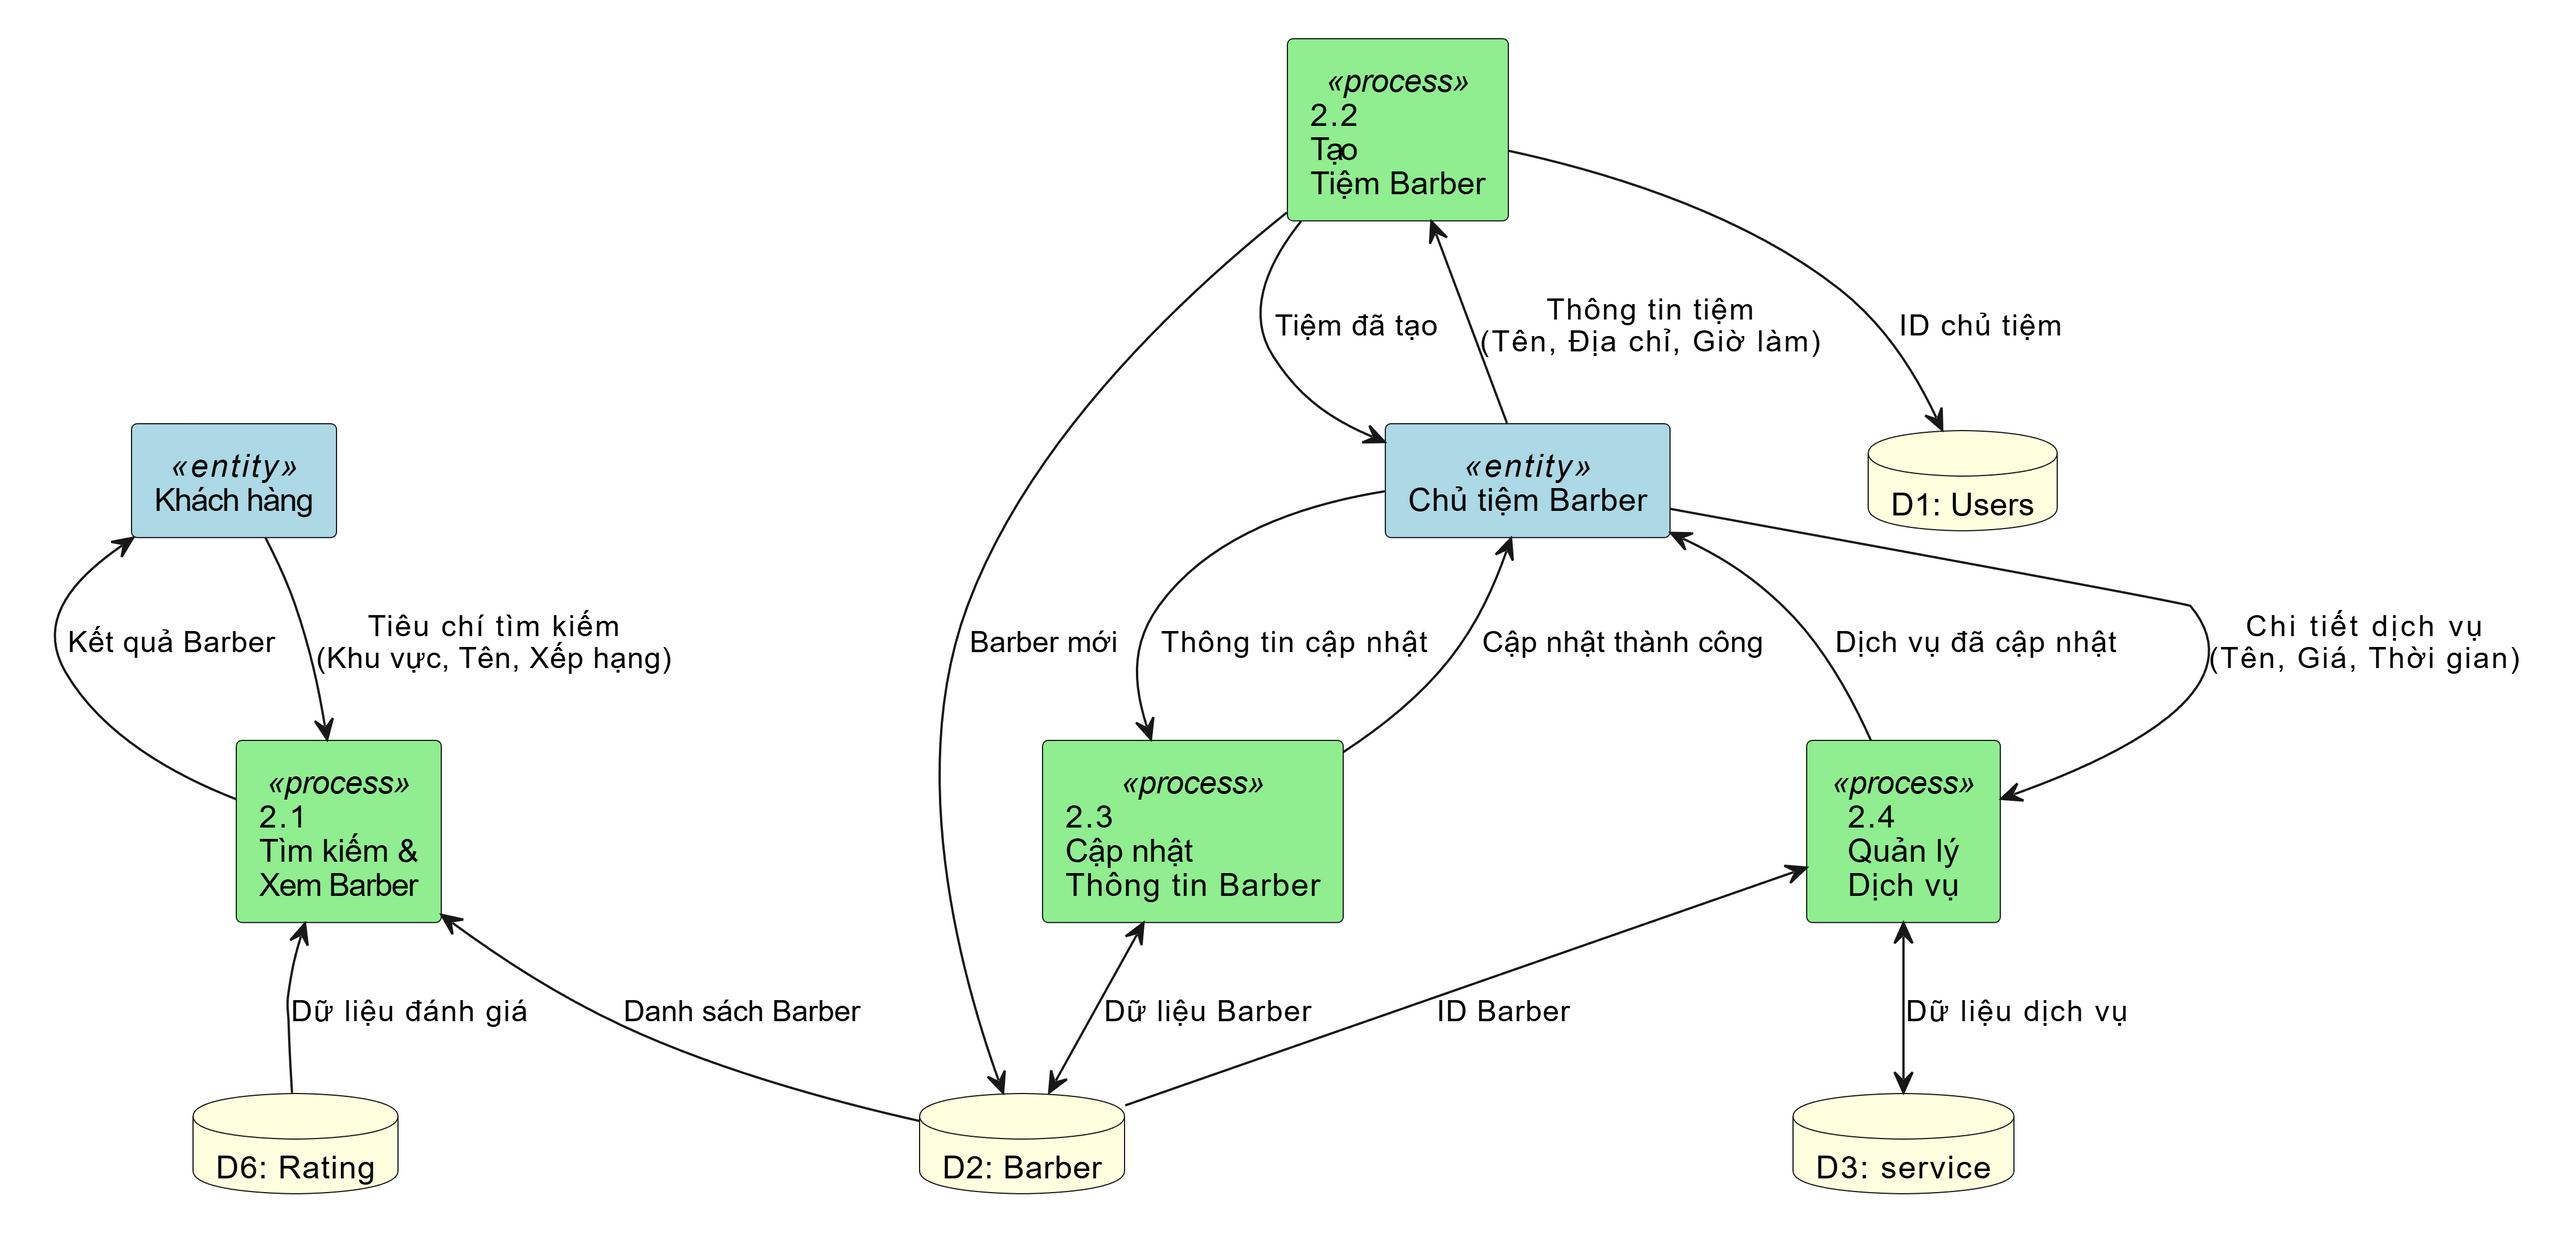
\includegraphics[width=0.7\textwidth]{figures/dfd1_mbarber.jpg}
    \caption{DFD cấp 1 - Quản lý cửa tiệm}
    \label{fig:dfd1_mbarber}
\end{figure}

Các tiến trình con:
\begin{itemize}
    \item \textbf{2.1 Tìm kiếm \& Xem Barber:} Khách hàng tìm kiếm tiệm cắt tóc theo khu vực, tên hoặc xếp hạng. Tiến trình truy vấn D2: Barbers và D6: Ratings để trả về kết quả phù hợp
    \item \textbf{2.2 Tạo Tiệm Barber:} Barber owner tạo tiệm mới với thông tin tên, địa chỉ, giờ làm việc. Hệ thống lấy ID người dùng từ D1: Users và tạo bản ghi mới trong D2: Barbers
    \item \textbf{2.3 Cập nhật Thông tin Barber:} Cho phép barber owner chỉnh sửa thông tin tiệm (địa chỉ, số điện thoại, mô tả, hình ảnh)
    \item \textbf{2.4 Quản lý Dịch vụ:} Barber owner thêm, sửa, xóa dịch vụ với thông tin tên, giá và thời gian thực hiện. Dữ liệu được lưu vào D3: Services và liên kết với barber ID từ D2: Barbers
\end{itemize}

\subsection{DFD cấp 1 - Quản lý đặt lịch}

DFD cấp 1 cho module Quản lý Đặt lịch mô tả quy trình từ xem khung giờ trống đến xác nhận và hủy lịch hẹn.

\begin{figure}[H]
    \centering
    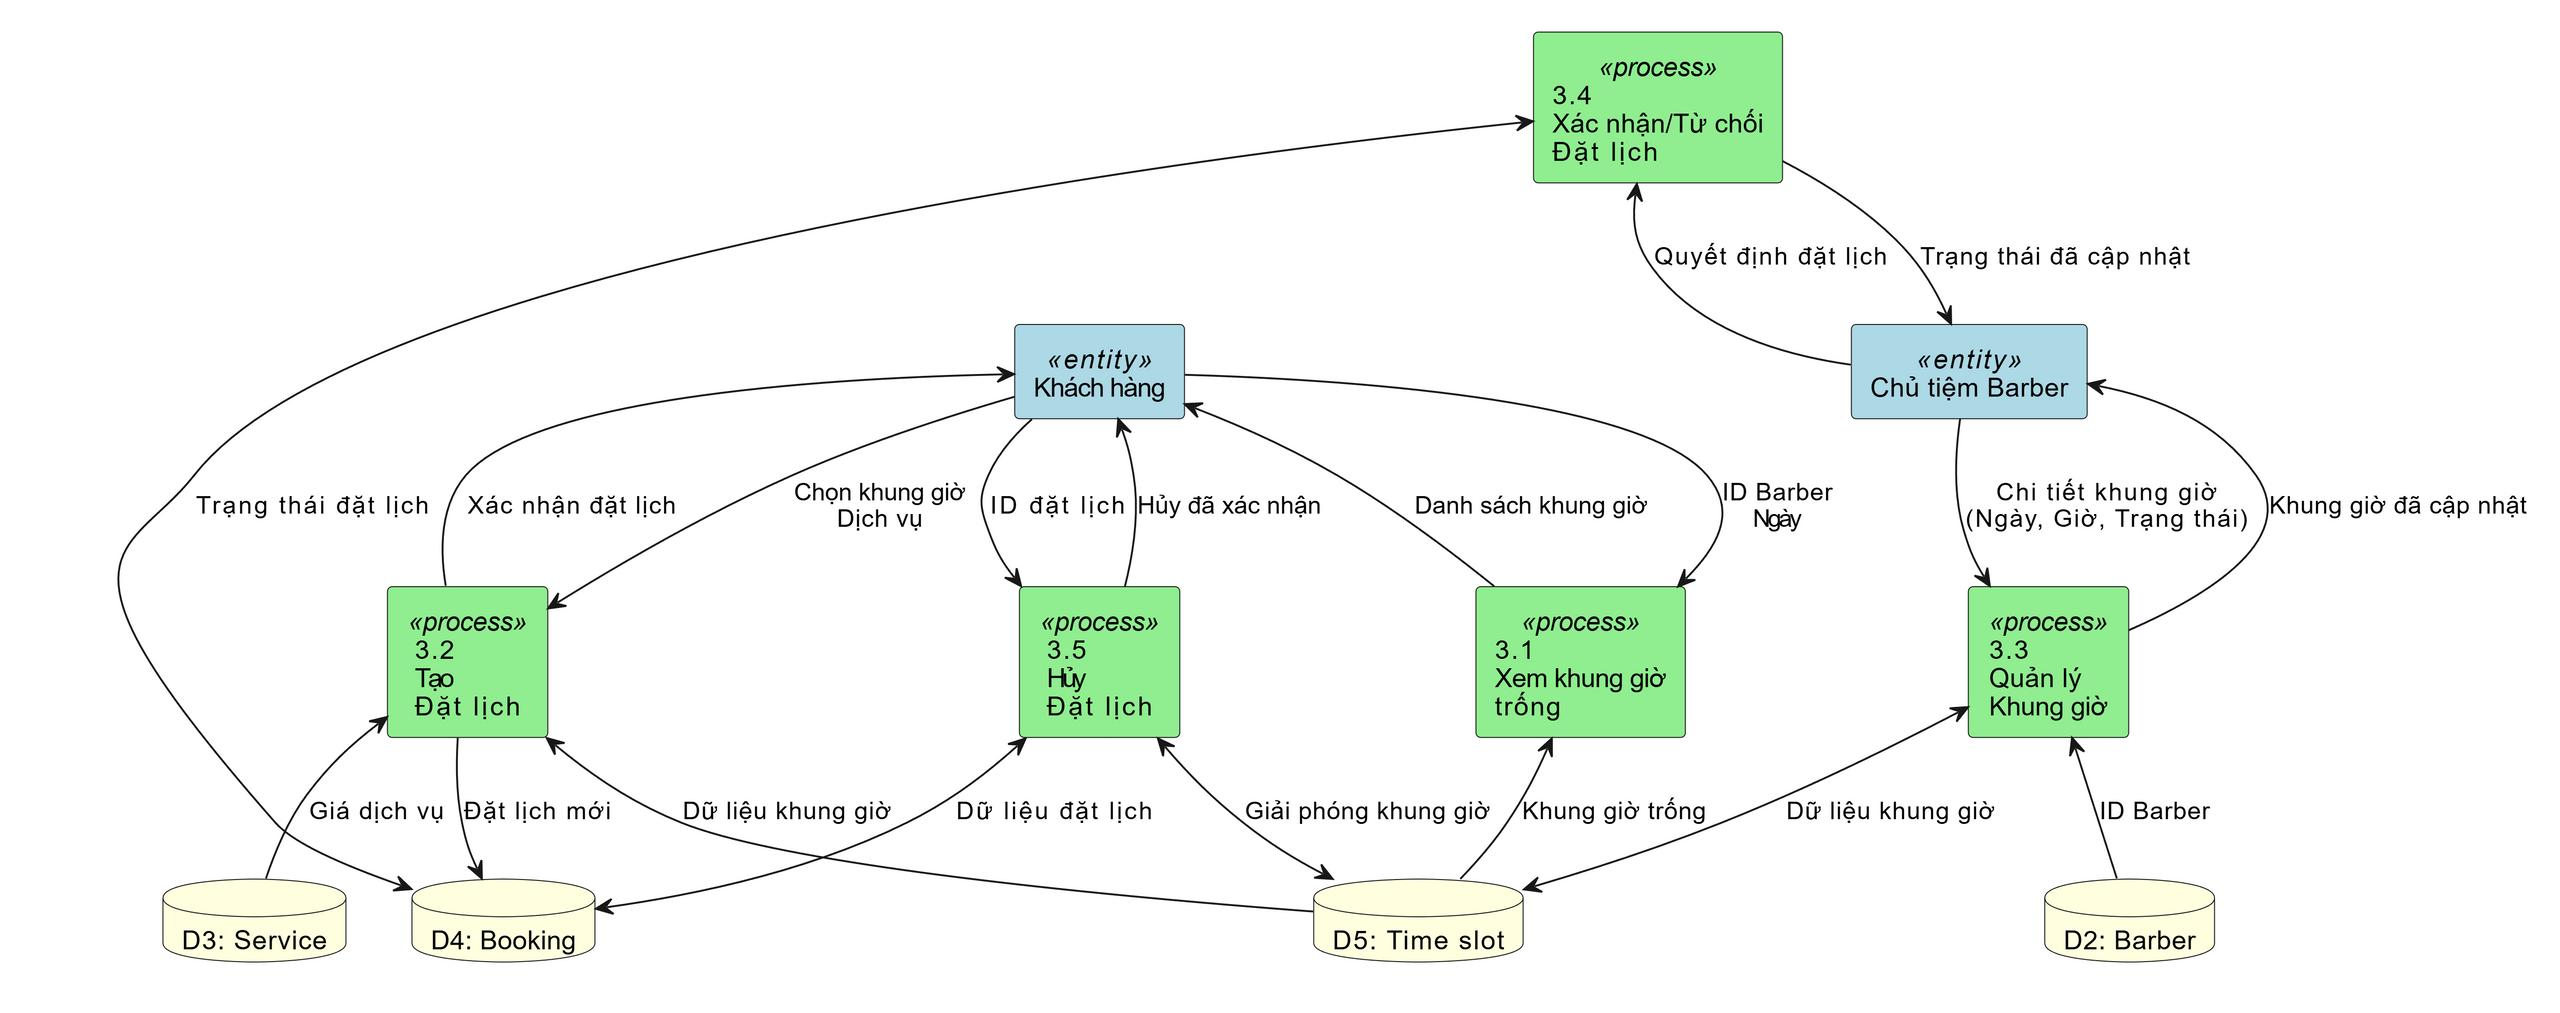
\includegraphics[width=0.8\textwidth]{figures/dfd1_book.jpg}
    \caption{DFD cấp 1 - Quản lý đặt lịch}
    \label{fig:dfd1_book}
\end{figure}

Các tiến trình con:
\begin{itemize}
    \item \textbf{3.1 Xem khung giờ trống:} Khách hàng chọn barber và ngày, hệ thống truy vấn D5: Time Slots để hiển thị các khung giờ còn trống
    \item \textbf{3.2 Tạo Đặt lịch:} Khách hàng chọn khung giờ và dịch vụ. Hệ thống tính tổng chi phí từ D3: Services, tạo booking mới trong D4: Bookings và cập nhật trạng thái khung giờ trong D5: Time Slots
    \item \textbf{3.3 Quản lý Khung giờ:} Barber owner tạo và cập nhật các khung giờ làm việc (ngày, giờ bắt đầu, giờ kết thúc, trạng thái available/booked)
    \item \textbf{3.4 Xác nhận/Từ chối Đặt lịch:} Barber owner xem danh sách booking và thay đổi trạng thái (confirmed/rejected) trong D4: Bookings
    \item \textbf{3.5 Hủy Đặt lịch:} Khách hàng có thể hủy lịch hẹn. Hệ thống cập nhật trạng thái trong D4: Bookings và giải phóng khung giờ trong D5: Time Slots
\end{itemize}

\subsection{DFD cấp 1 - Quản lý đánh giá}

DFD cấp 1 cho module Đánh giá mô tả cách khách hàng đánh giá dịch vụ và cách hệ thống tính toán xếp hạng trung bình.

\begin{figure}[H]
    \centering
    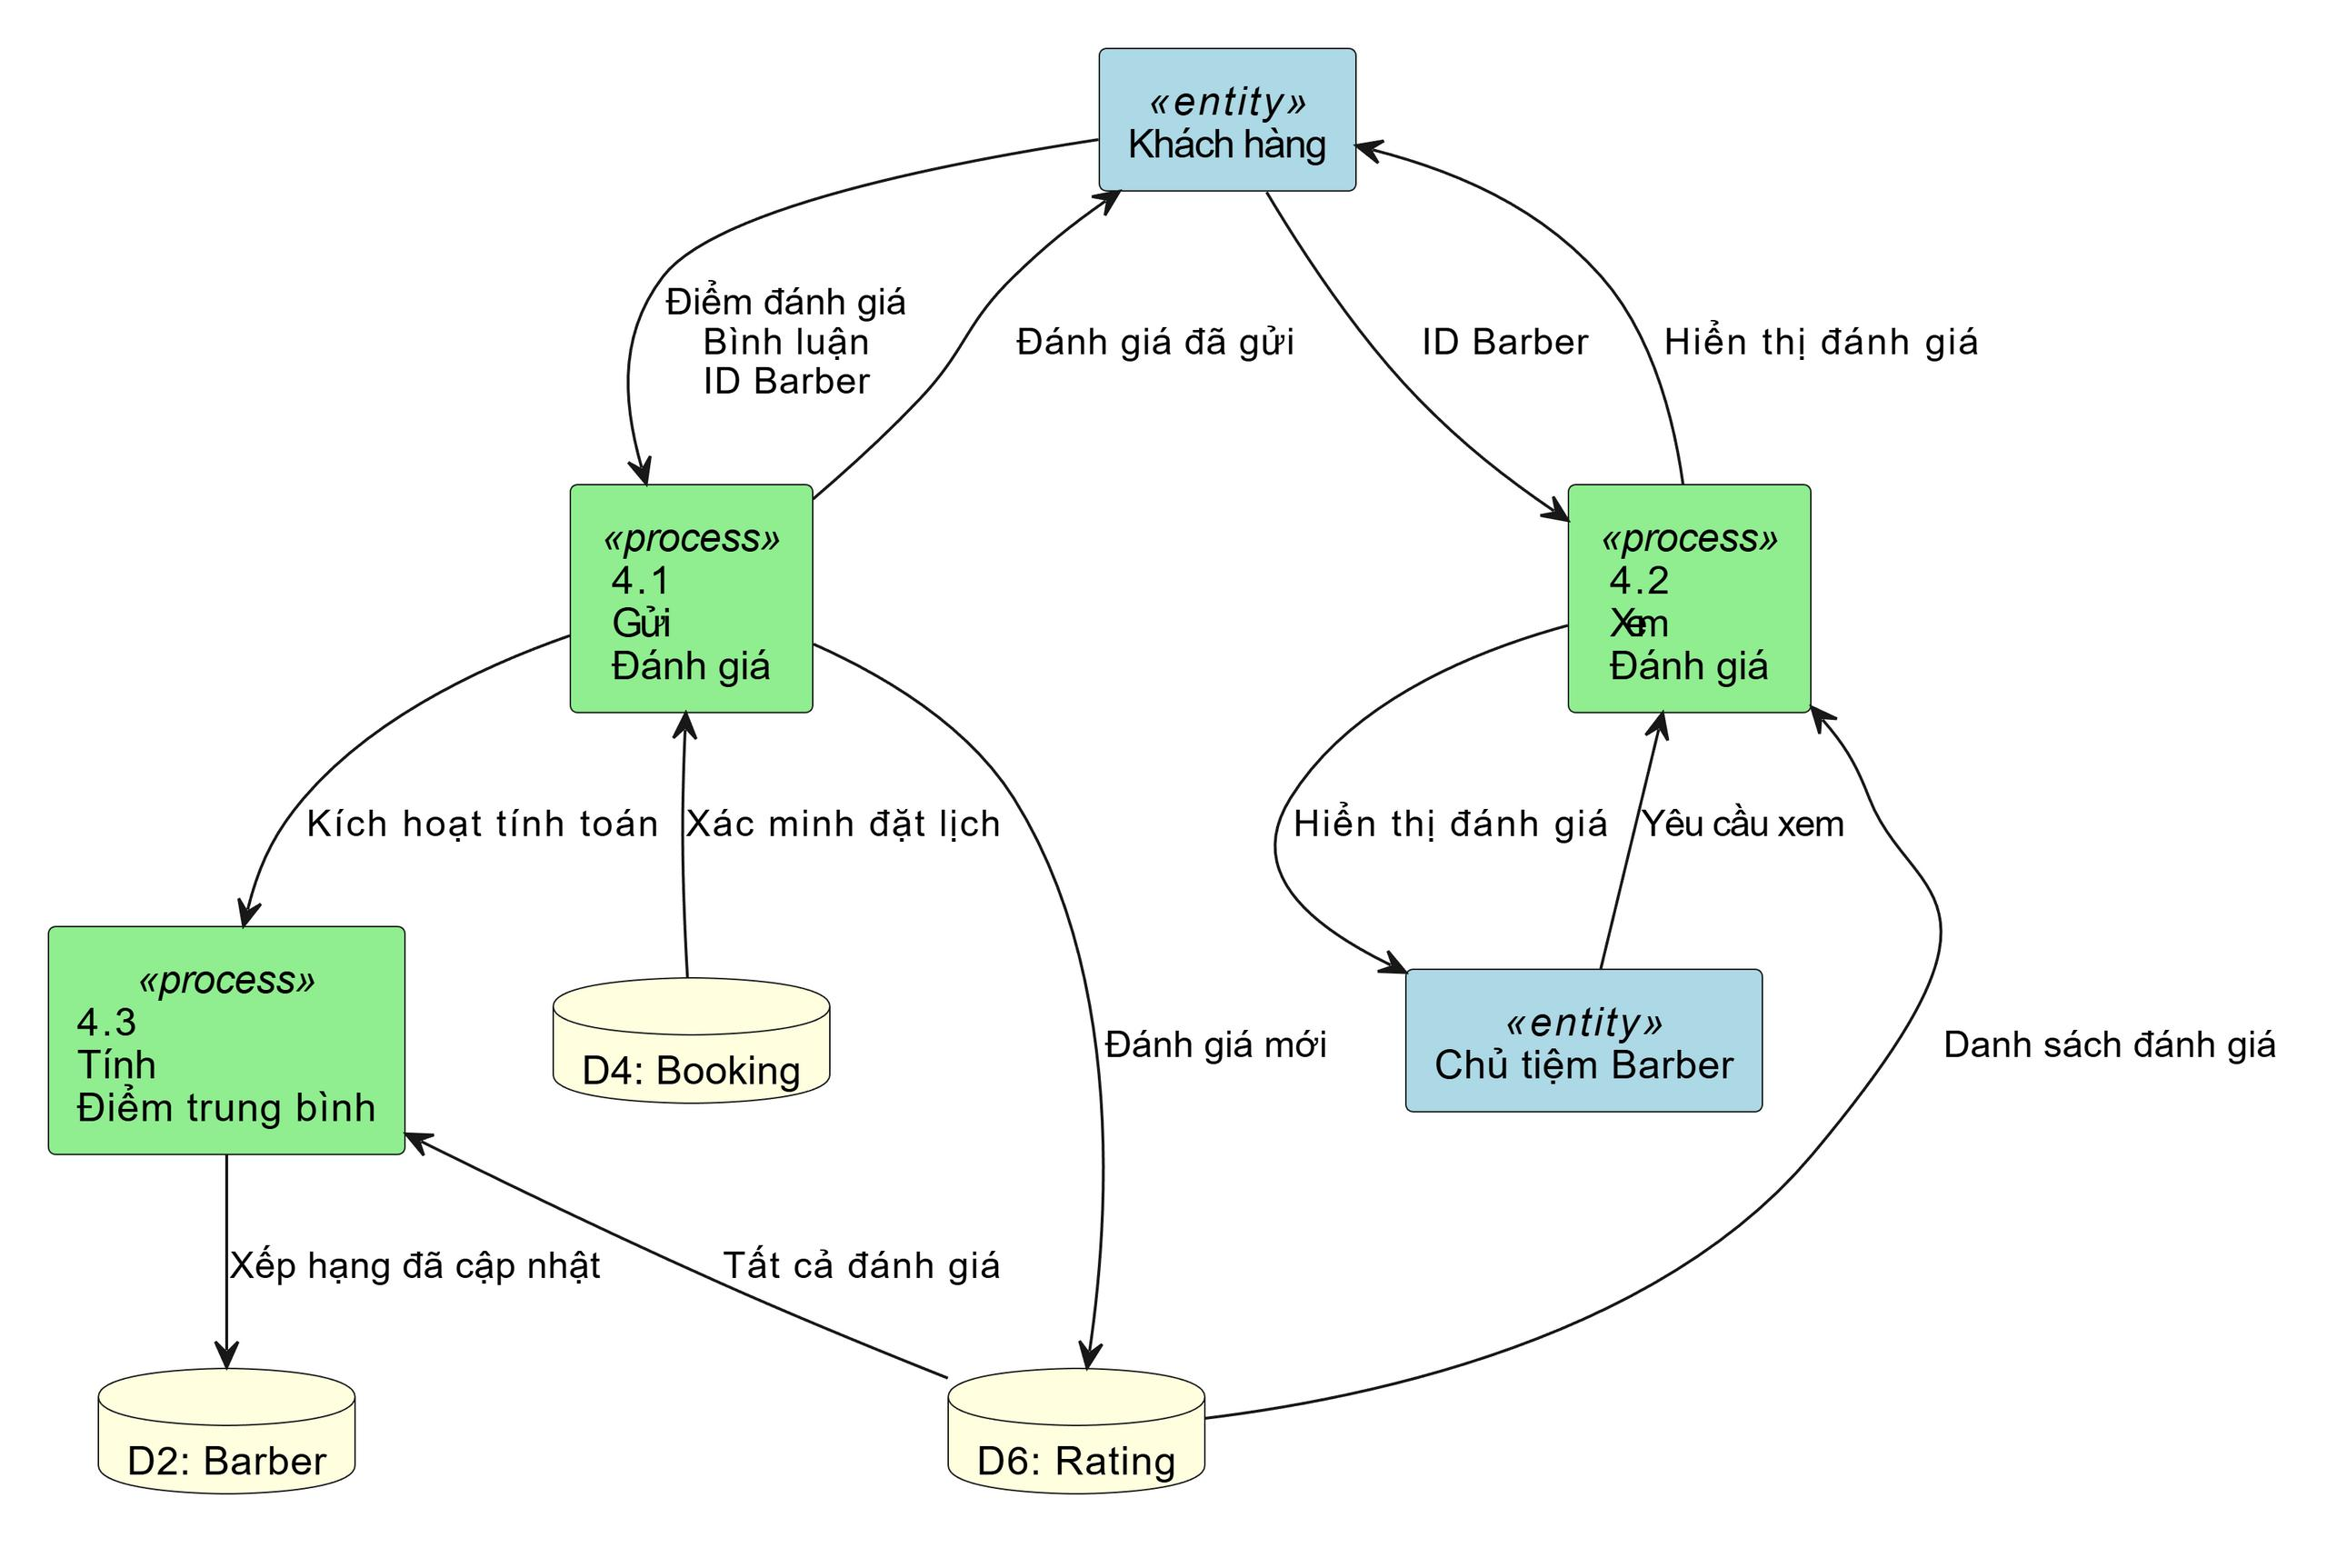
\includegraphics[width=0.7\textwidth]{figures/dfd1_rating.jpg}
    \caption{DFD cấp 1 - Quản lý đánh giá}
    \label{fig:dfd1_rating}
\end{figure}

Các tiến trình con:
\begin{itemize}
    \item \textbf{4.1 Gửi Đánh giá:} Khách hàng gửi đánh giá sau khi sử dụng dịch vụ (điểm số 1-5 sao và bình luận). Hệ thống xác minh booking hoàn thành từ D4: Bookings trước khi lưu vào D6: Ratings, sau đó kích hoạt tiến trình 4.3
    \item \textbf{4.2 Xem Đánh giá:} Khách hàng và barber owner xem danh sách đánh giá của một tiệm cụ thể từ D6: Ratings
    \item \textbf{4.3 Tính Điểm trung bình:} Được kích hoạt tự động khi có đánh giá mới. Tiến trình lấy tất cả đánh giá từ D6: Ratings, tính điểm trung bình và cập nhật xếp hạng vào D2: Barbers
\end{itemize}

\subsection{DFD cấp 1 - Tính năng AI}

DFD cấp 1 cho module AI Features chi tiết hóa các tiến trình xử lý phát hiện mụn, tạo kiểu tóc và chatbot RAG.

\begin{figure}[H]
    \centering
    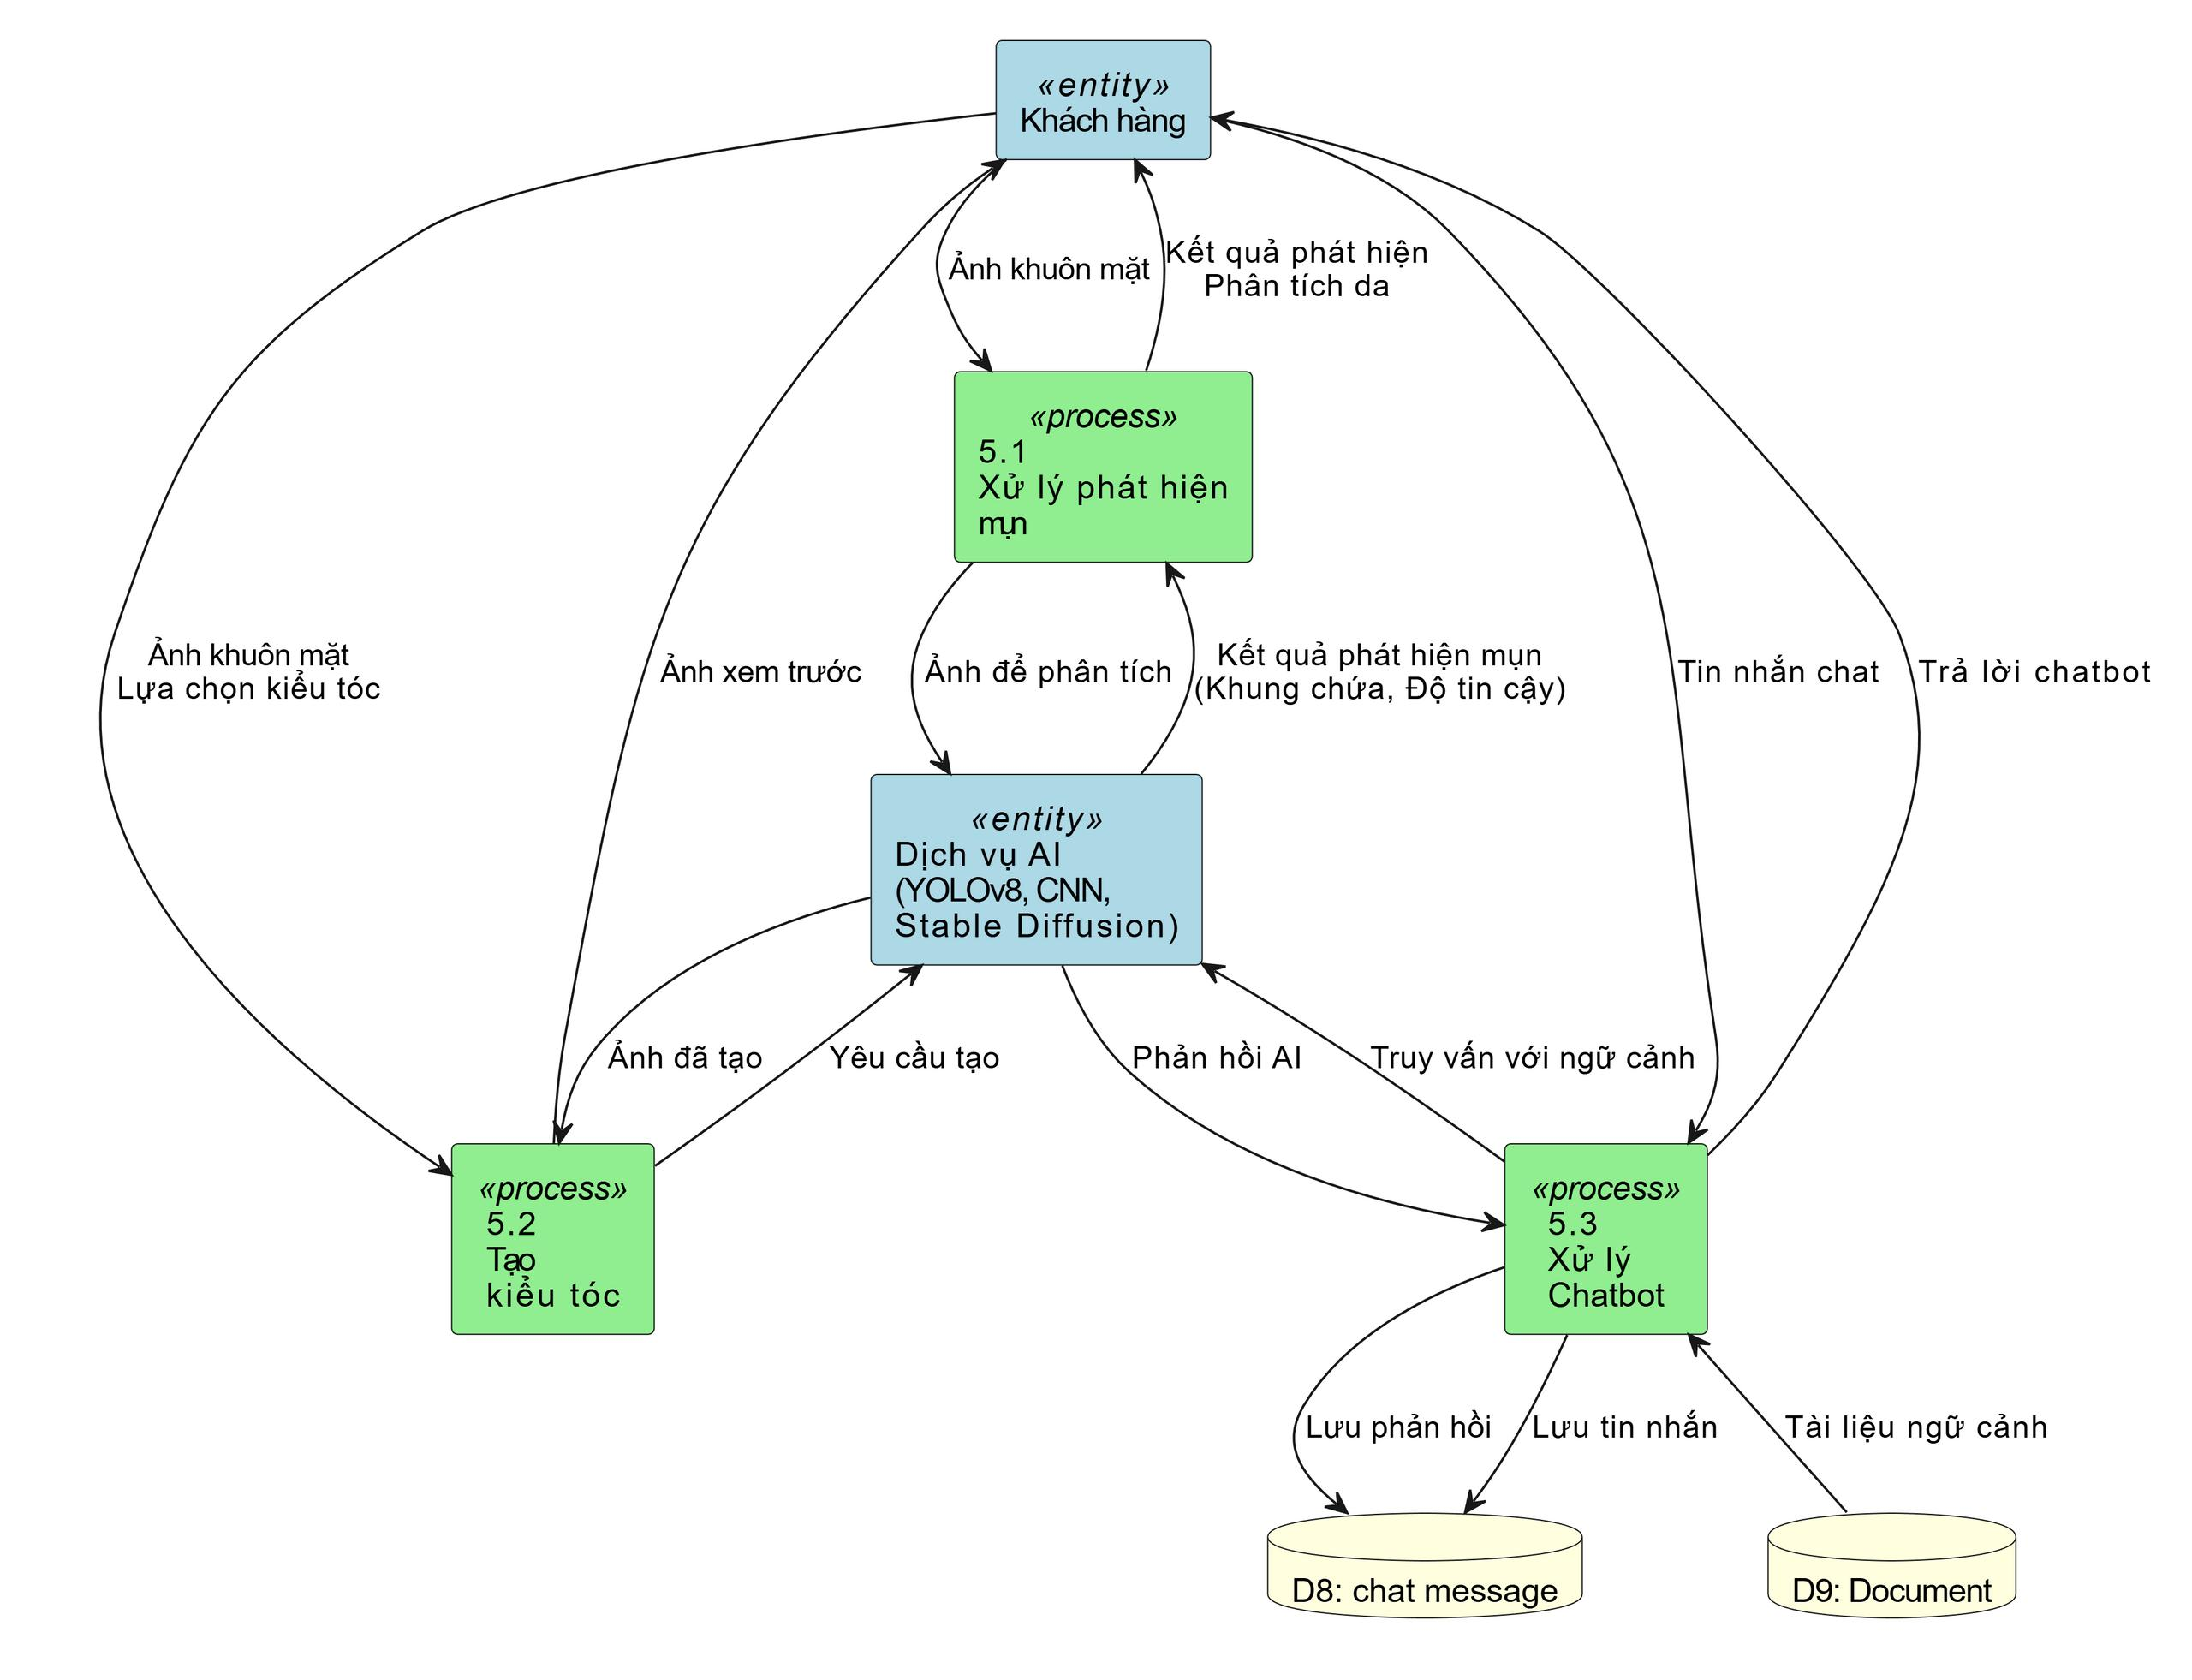
\includegraphics[width=0.8\textwidth]{figures/dfd1_ai.jpg}
    \caption{DFD cấp 1 - Tính năng AI}
    \label{fig:dfd1_ai}
\end{figure}

Các tiến trình con:
\begin{itemize}
    \item \textbf{5.1 Xử lý phát hiện mụn:} Khách hàng upload ảnh khuôn mặt. Hệ thống gửi ảnh đến AI Service (YOLOv8 + CNN) để phân tích. AI trả về kết quả phát hiện với bounding boxes và độ tin cậy. Hệ thống tổng hợp và trả kết quả phân tích da cho khách hàng
    \item \textbf{5.2 Tạo kiểu tóc:} Khách hàng upload ảnh và chọn kiểu tóc mong muốn. Hệ thống gửi request đến AI Service (Stable Diffusion Inpainting). AI tạo ảnh mới với kiểu tóc đã chọn và trả về cho khách hàng xem trước
    \item \textbf{5.3 Xử lý Chatbot:} Khách hàng gửi tin nhắn chat. Hệ thống lưu tin nhắn vào D8: Chat Messages, truy vấn ngữ cảnh liên quan từ D9: Documents (RAG), gửi query cùng context đến AI Service (Gemini). AI trả về phản hồi, hệ thống lưu vào D8 và hiển thị cho khách hàng
\end{itemize}

\subsection{DFD cấp 1 - Quản lý Yêu cầu hợp tác}

DFD cấp 1 cho module Hợp tác mô tả quy trình từ khi khách hàng gửi yêu cầu đến khi admin phê duyệt/từ chối và gửi thông báo.

\begin{figure}[H]
    \centering
    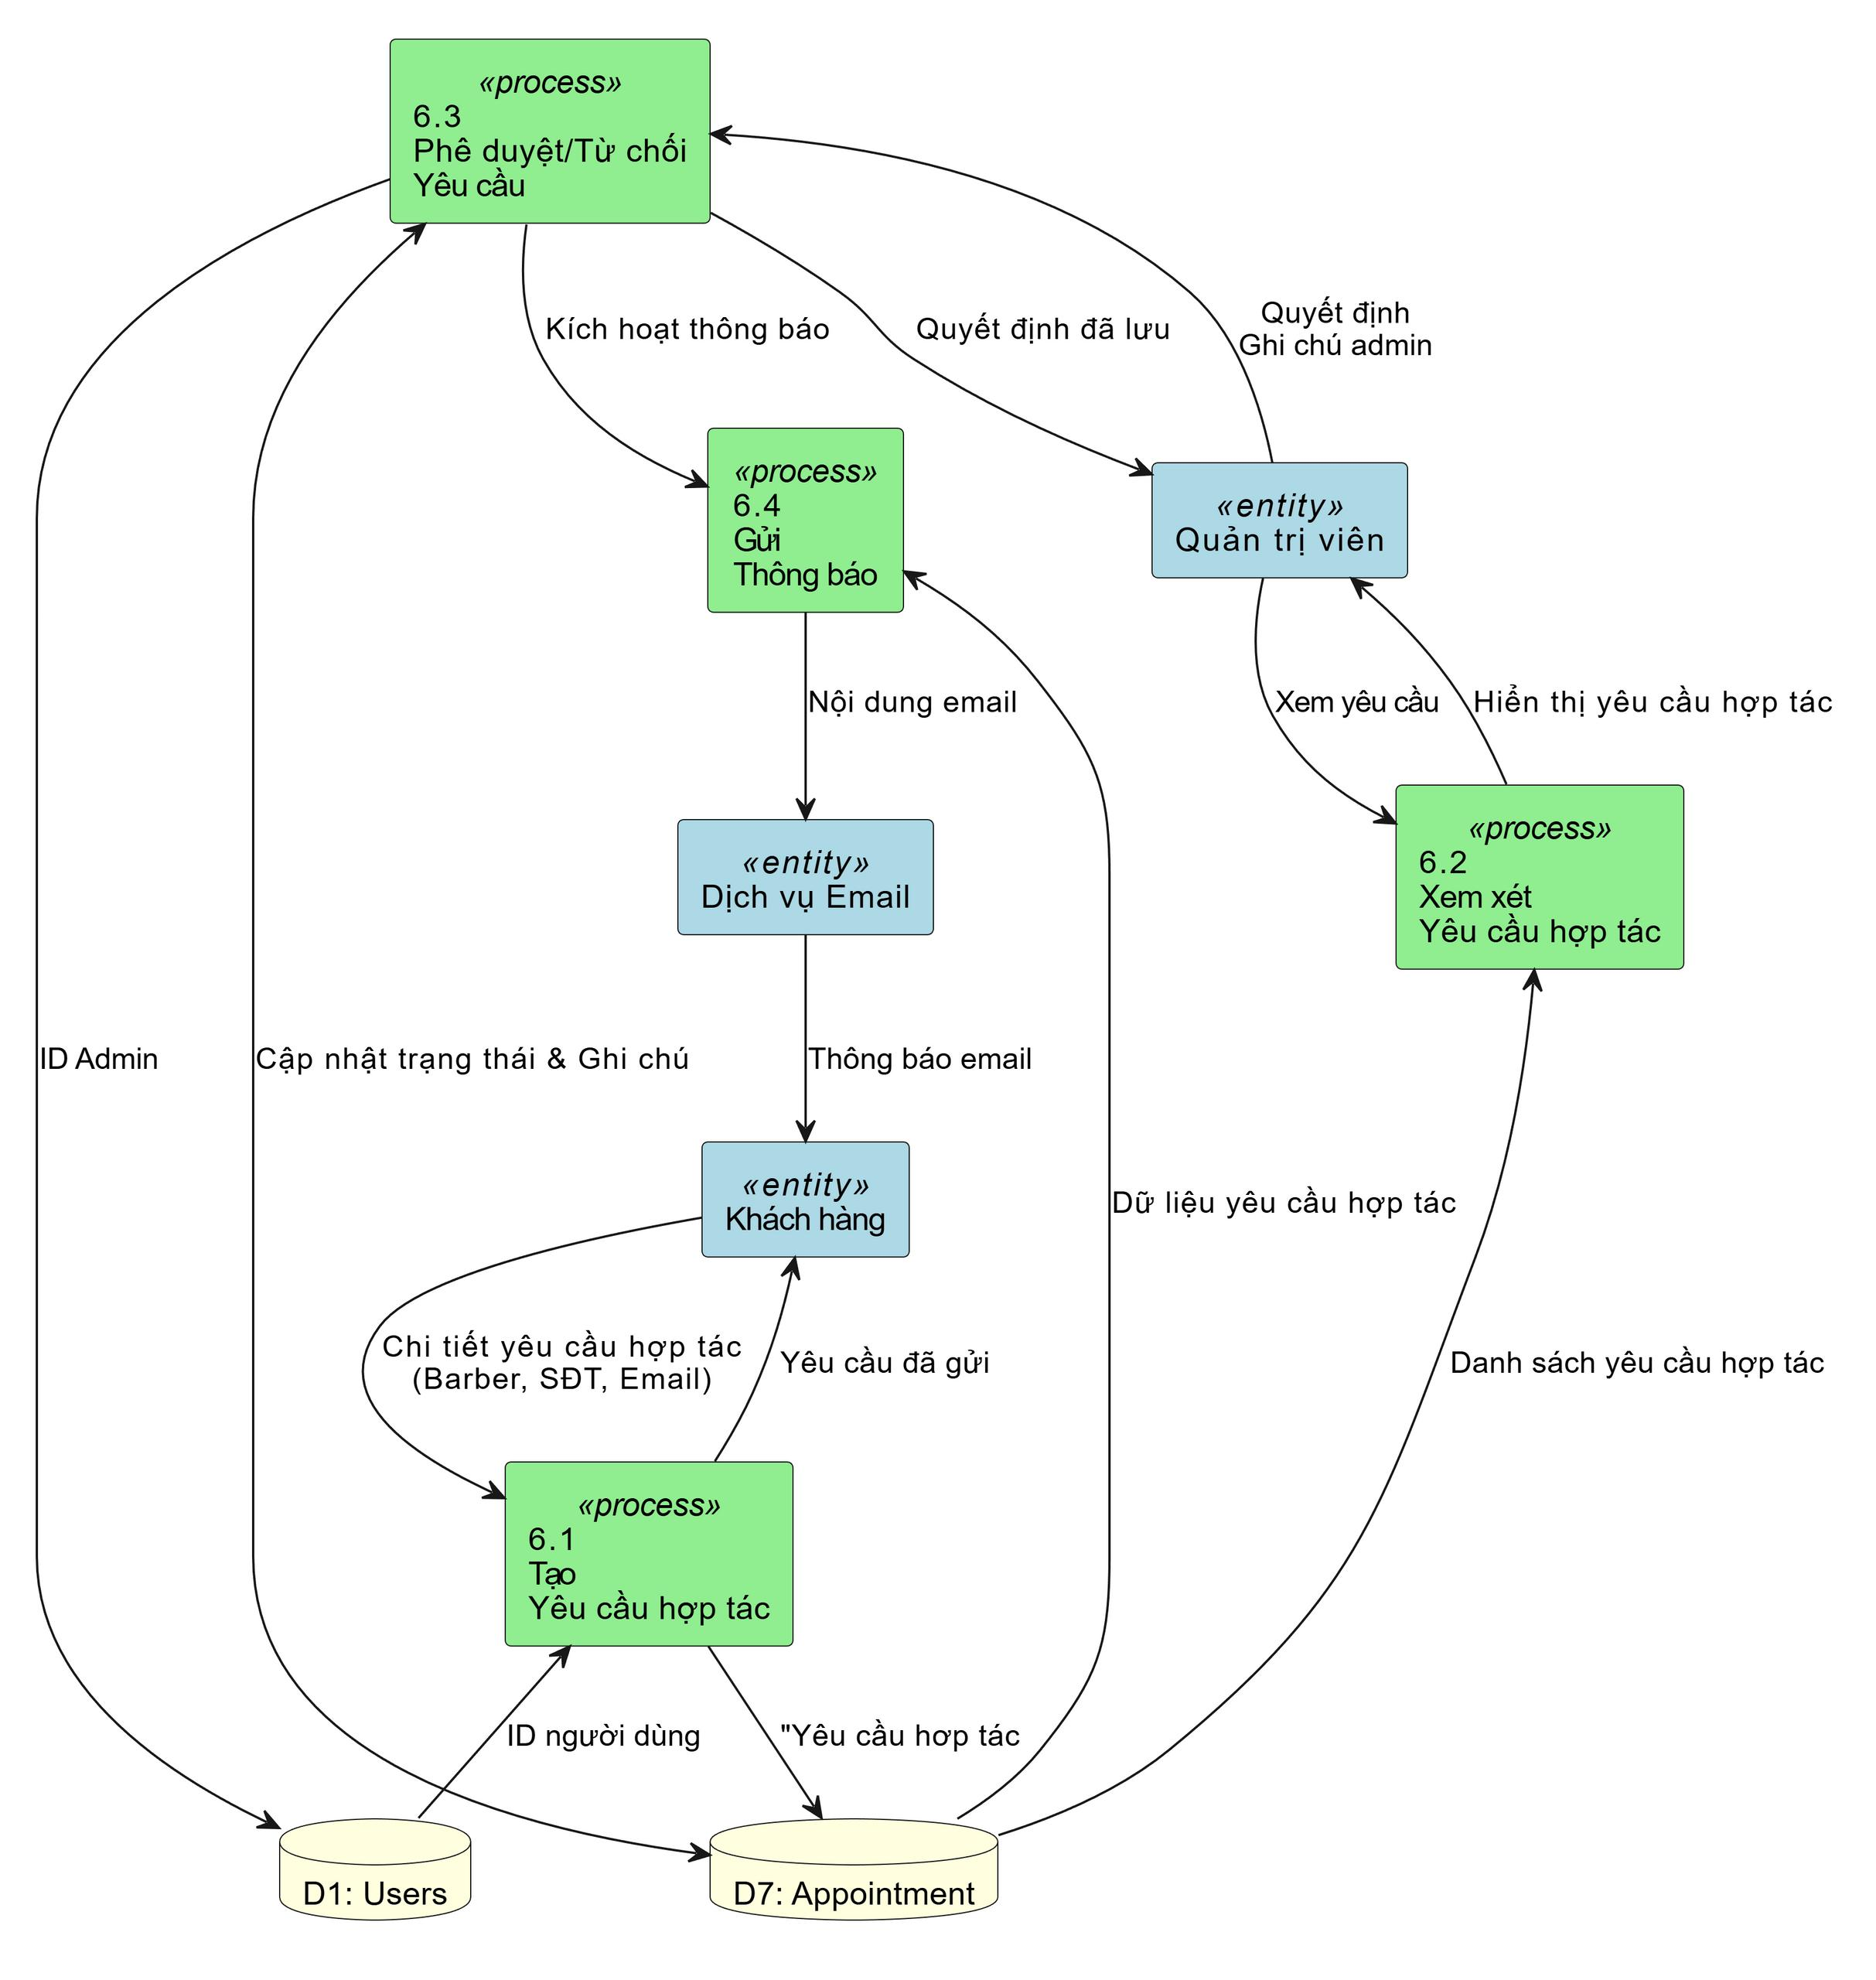
\includegraphics[width=0.8\textwidth]{figures/dfd1_req.jpg}
    \caption{DFD cấp 1 - Quản lý Yêu cầu hợp tác}
    \label{fig:dfd1_collab}
\end{figure}

Các tiến trình con:
\begin{itemize}
    \item \textbf{6.1 Tạo Yêu cầu hợp tác:} Khách hàng điền form yêu cầu hợp tác với thông tin barber shop muốn mở, số điện thoại, email liên hệ. Hệ thống lấy ID người dùng từ D1: Users và tạo bản ghi mới trong D7: Appointments với trạng thái "pending"
    \item \textbf{6.2 Xem xét Yêu cầu hợp tác:} Admin xem danh sách tất cả yêu cầu hợp tác từ D7: Appointments, có thể lọc theo trạng thái (pending/approved/rejected)
    \item \textbf{6.3 Phê duyệt/Từ chối Yêu cầu:} Admin xem chi tiết yêu cầu, thêm ghi chú quản trị và quyết định chấp nhận hoặc từ chối. Hệ thống cập nhật trạng thái và ghi chú vào D7: Appointments, lưu ID admin vào D1: Users và kích hoạt tiến trình 6.4
    \item \textbf{6.4 Gửi Thông báo:} Được kích hoạt tự động sau khi admin ra quyết định. Tiến trình lấy dữ liệu từ D7: Appointments, tạo nội dung email và gửi qua Email Service đến địa chỉ email của khách hàng
\end{itemize}

\subsection{DFD Cấp 1 - Hệ thống Thông báo}

DFD cấp 1 cho module Thông báo mô tả cách hệ thống tạo và gửi thông báo đẩy đến thiết bị di động của người dùng.

\begin{figure}[H]
    \centering
    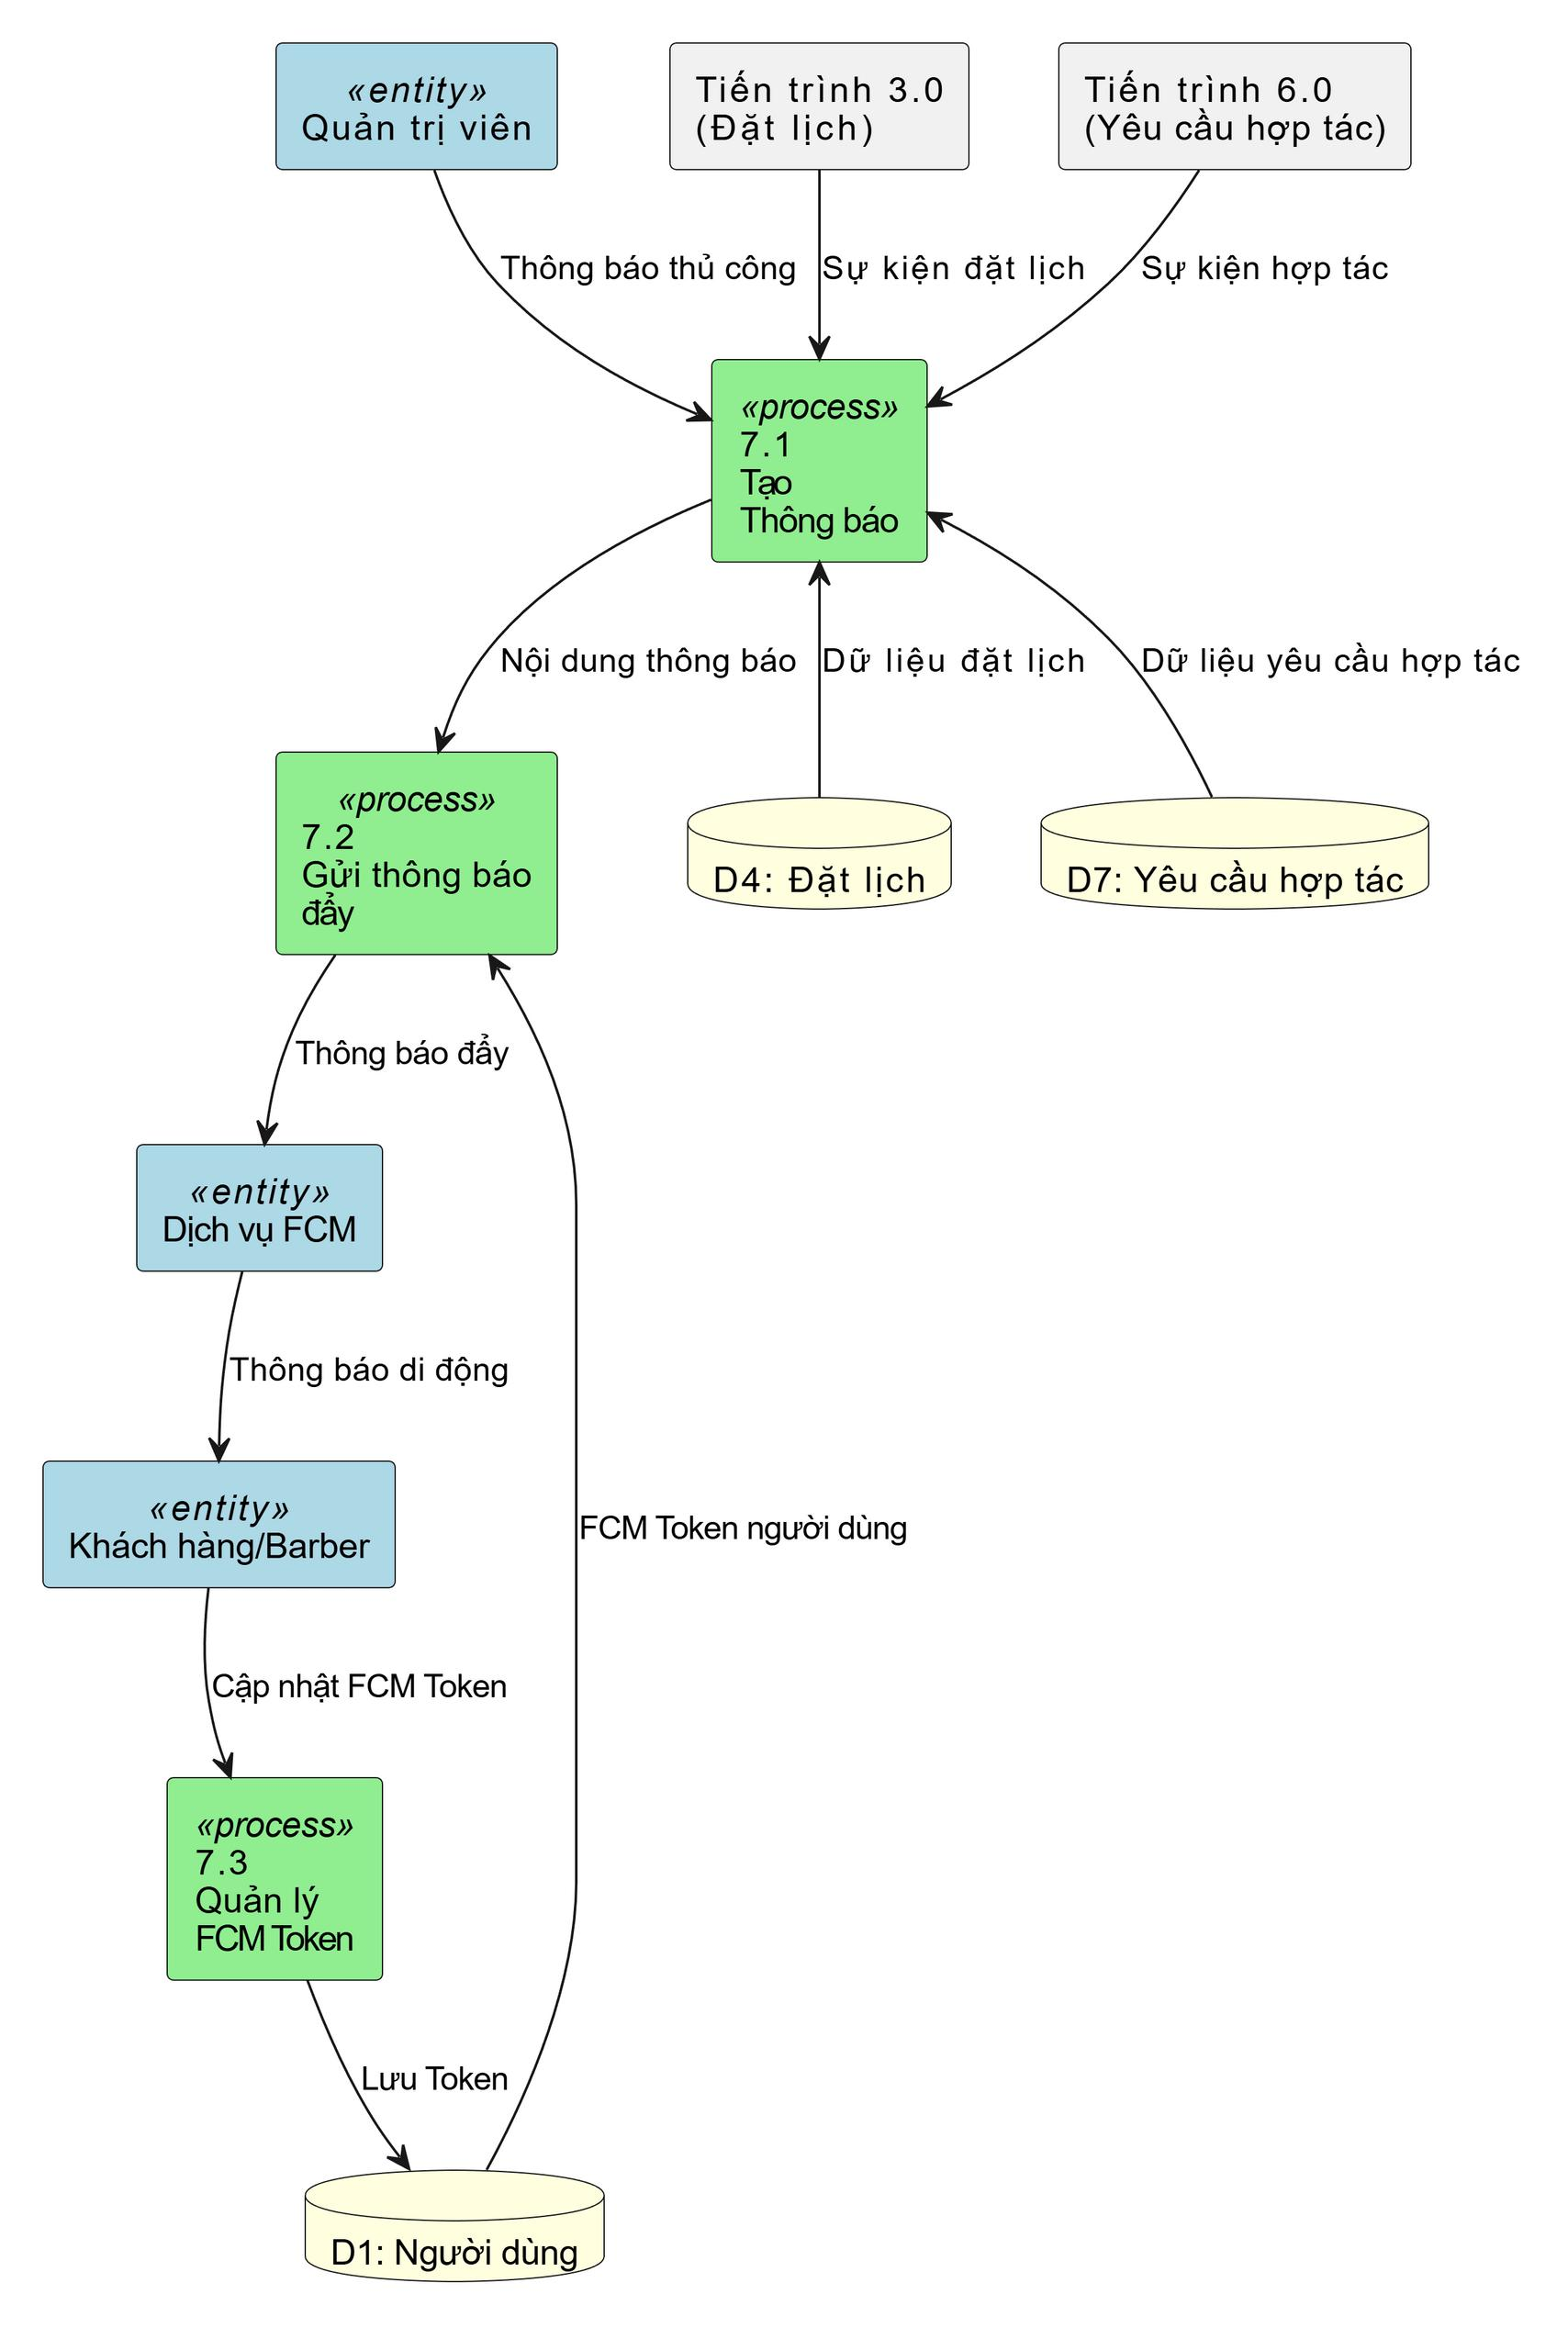
\includegraphics[width=0.8\textwidth]{figures/dfd1_noti.jpg}
    \caption{DFD cấp 1 - Hệ thống Thông báo}
    \label{fig:dfd1_noti}
\end{figure}

Các tiến trình con:
\begin{itemize}
    \item \textbf{7.1 Tạo Thông báo:} Nhận sự kiện từ Tiến trình 3.0 (Đặt lịch) hoặc Tiến trình 6.0 (Yêu cầu hợp tác), hoặc thông báo thủ công từ admin. Tiến trình truy vấn dữ liệu liên quan từ D4: Bookings và D7: Appointments để tạo nội dung thông báo phù hợp
    \item \textbf{7.2 Gửi thông báo đẩy:} Nhận nội dung thông báo từ 7.1, truy vấn FCM token từ D1: Users của người nhận, gửi push notification qua Firebase Cloud Messaging (FCM). FCM Service phân phối thông báo đến thiết bị di động của người dùng
    \item \textbf{7.3 Quản lý FCM Token:} Khi người dùng đăng nhập/đăng xuất hoặc cài đặt/gỡ ứng dụng, thiết bị gửi FCM token mới hoặc yêu cầu xóa token. Tiến trình cập nhật token vào D1: Users để đảm bảo thông báo được gửi đến đúng thiết bị
\end{itemize}